\documentclass[12pt]{article}
\usepackage[margin=1in]{geometry}
\usepackage{graphicx}
\usepackage{subcaption}
\usepackage{booktabs}
\usepackage{hyperref}

\title{Alzheimer's MRI Classification --- Figures\\
\large ResNet-10 vs ResNet-18}
\author{}
\date{}

\begin{document}
\maketitle
\tableofcontents
\newpage

%%% ─────────────────────────────────────────────────────────
\section{Training Curves}

\begin{figure}[h]
  \centering
  \begin{subfigure}[b]{0.48\textwidth}
    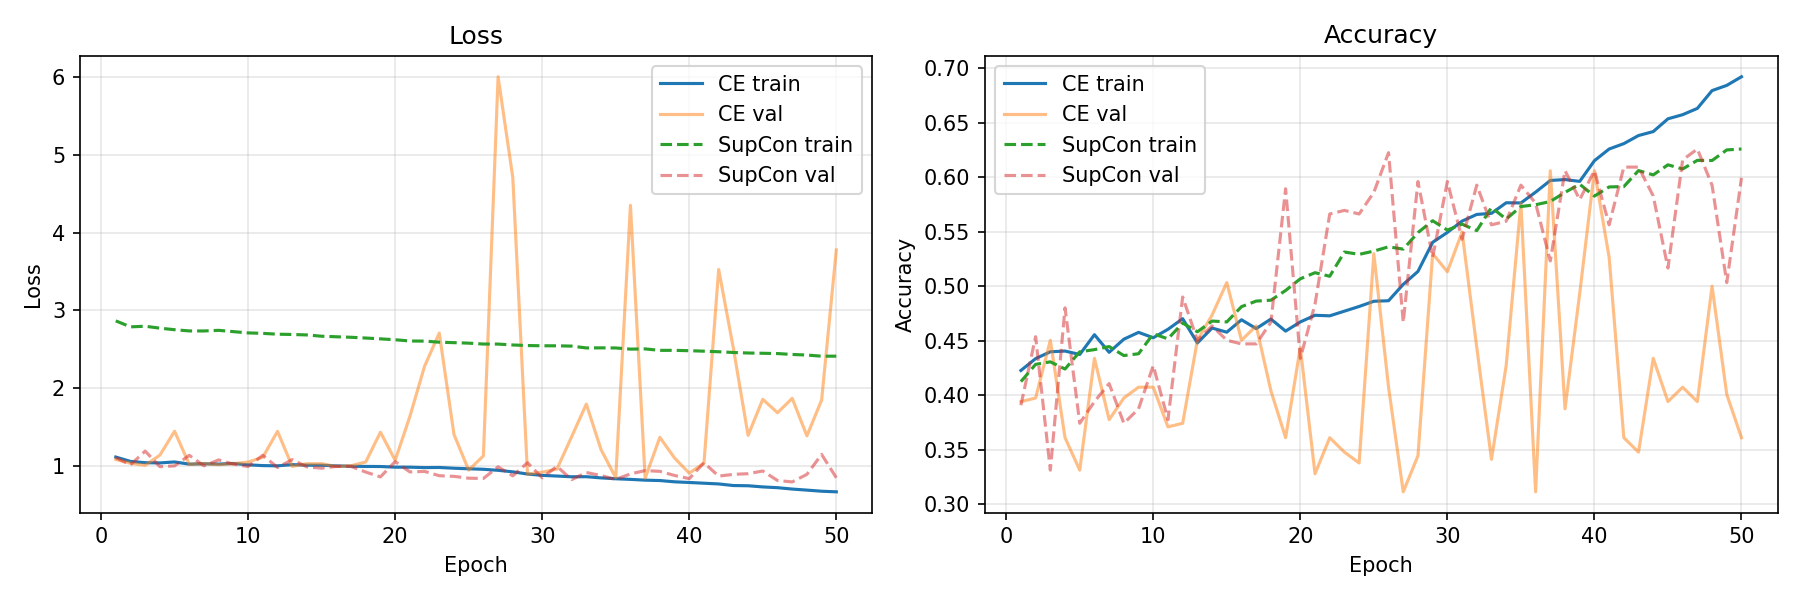
\includegraphics[width=\textwidth]{resnet10/training_curves.png}
    \caption{ResNet-10}
  \end{subfigure}
  \hfill
  \begin{subfigure}[b]{0.48\textwidth}
    
\includegraphics[width=\textwidth]{resnet18/training_curves.png}
    \caption{ResNet-18}
  \end{subfigure}
  \caption{Training and validation loss/accuracy curves for CE and SupCon runs.}
  \label{fig:training_curves}
\end{figure}

%%% ─────────────────────────────────────────────────────────
\section{CE vs.\ SupCon Comparison}

\begin{figure}[h]
  \centering
  \begin{subfigure}[b]{0.48\textwidth}
    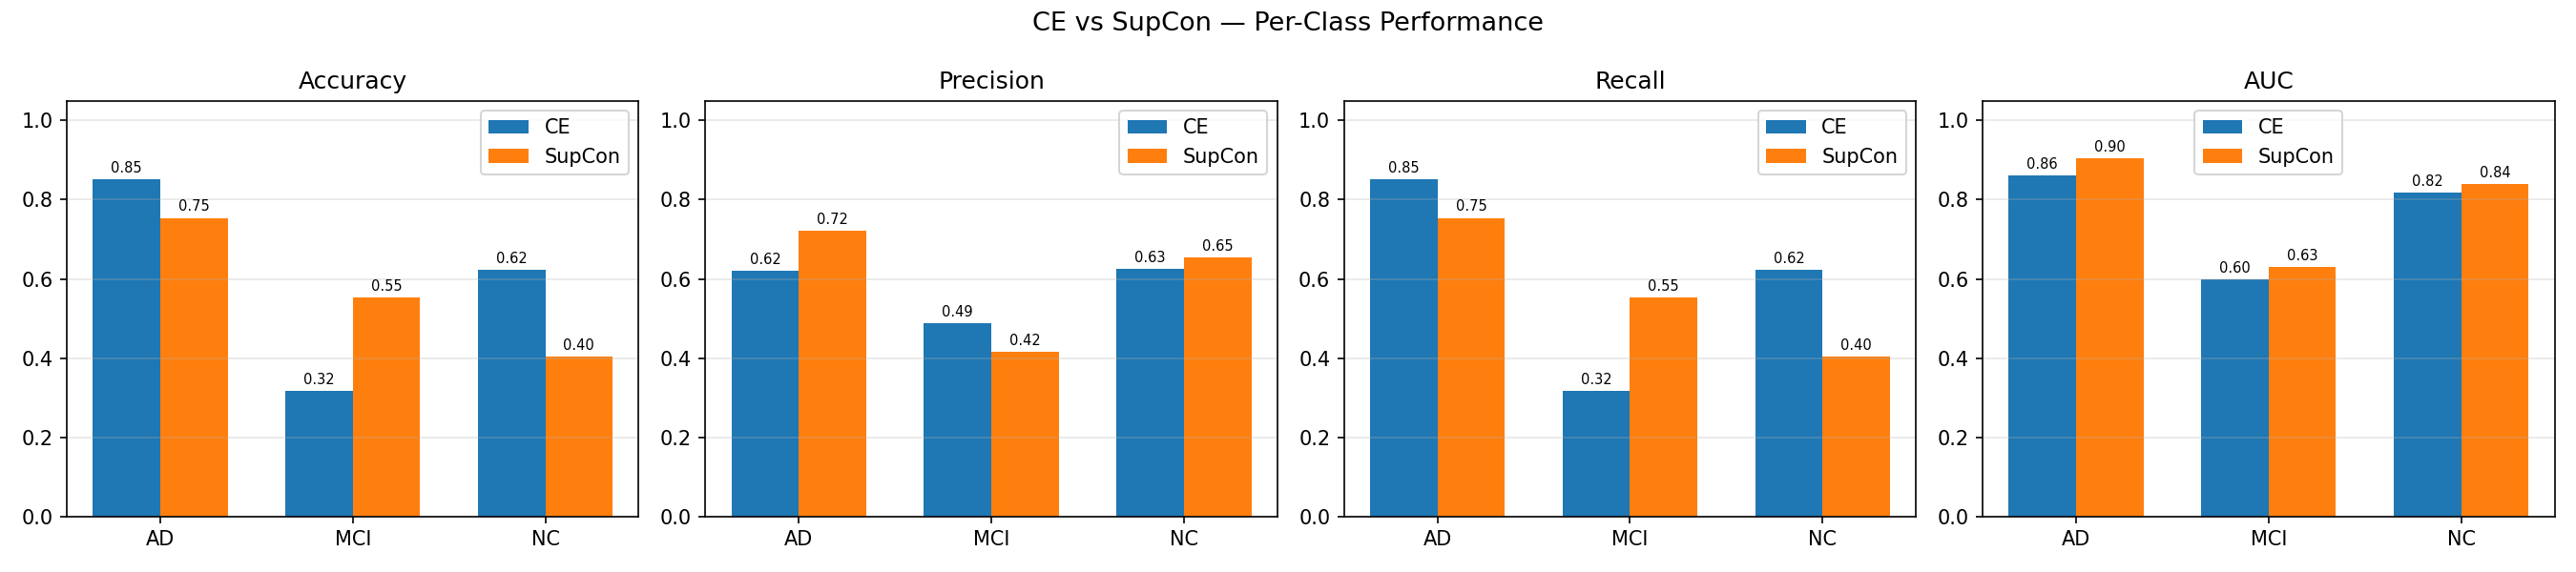
\includegraphics[width=\textwidth]{resnet10/comparison.png}
    \caption{ResNet-10}
  \end{subfigure}
  \hfill
  \begin{subfigure}[b]{0.48\textwidth}
    
\includegraphics[width=\textwidth]{resnet18/comparison.png}
    \caption{ResNet-18}
  \end{subfigure}
  \caption{Side-by-side metric comparison between cross-entropy (CE) and supervised contrastive (SupCon) training.}
  \label{fig:comparison}
\end{figure}

%%% ─────────────────────────────────────────────────────────
\section{Confusion Matrices}

\subsection{Cross-Entropy}

\begin{figure}[h]
  \centering
  \begin{subfigure}[b]{0.48\textwidth}
    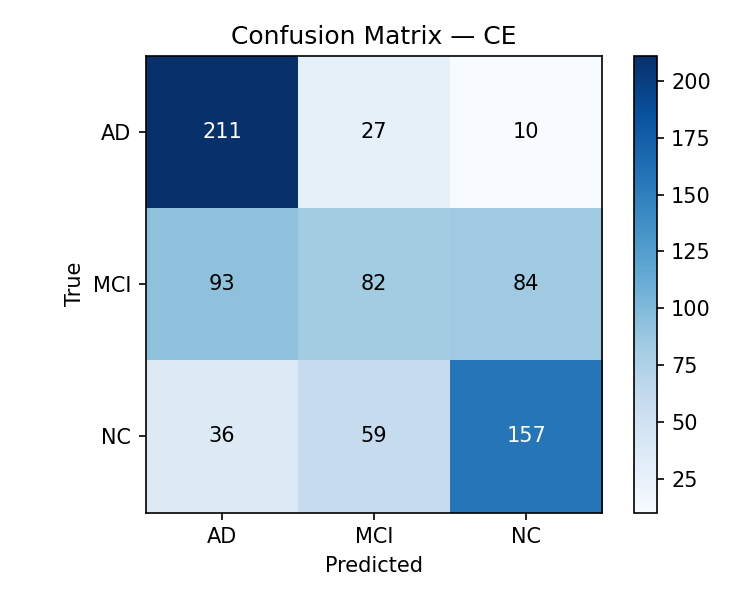
\includegraphics[width=\textwidth]{resnet10/cm_ce.png}
    \caption{ResNet-10 CE}
  \end{subfigure}
  \hfill
  \begin{subfigure}[b]{0.48\textwidth}
    
\includegraphics[width=\textwidth]{resnet18/cm_ce.png}
    \caption{ResNet-18 CE}
  \end{subfigure}
  \caption{Confusion matrices for the cross-entropy baseline.}
  \label{fig:cm_ce}
\end{figure}

\subsection{Supervised Contrastive}

\begin{figure}[h]
  \centering
  \begin{subfigure}[b]{0.48\textwidth}
    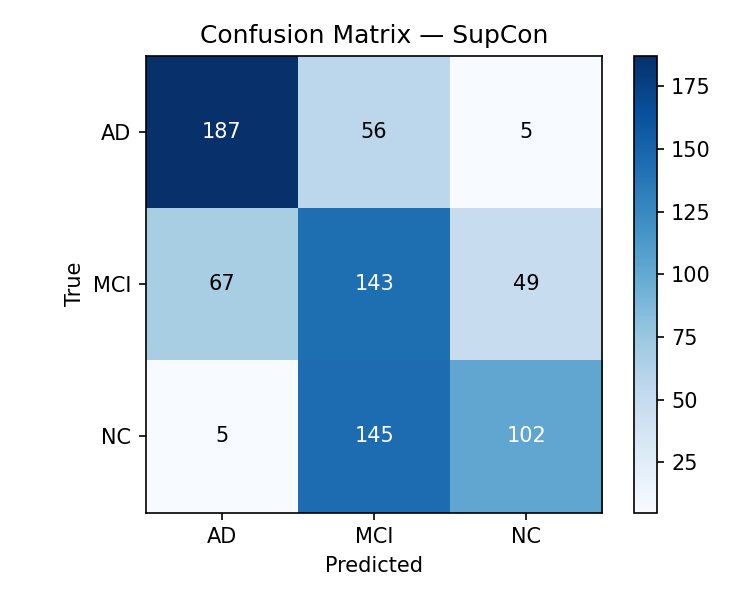
\includegraphics[width=\textwidth]{resnet10/cm_supcon.png}
    \caption{ResNet-10 SupCon}
  \end{subfigure}
  \hfill
  \begin{subfigure}[b]{0.48\textwidth}
    
\includegraphics[width=\textwidth]{resnet18/cm_supcon.png}
    \caption{ResNet-18 SupCon}
  \end{subfigure}
  \caption{Confusion matrices for supervised contrastive training.}
  \label{fig:cm_supcon}
\end{figure}

%%% ─────────────────────────────────────────────────────────
\section{ROC Curves}

\subsection{Cross-Entropy}

\begin{figure}[h]
  \centering
  \begin{subfigure}[b]{0.48\textwidth}
    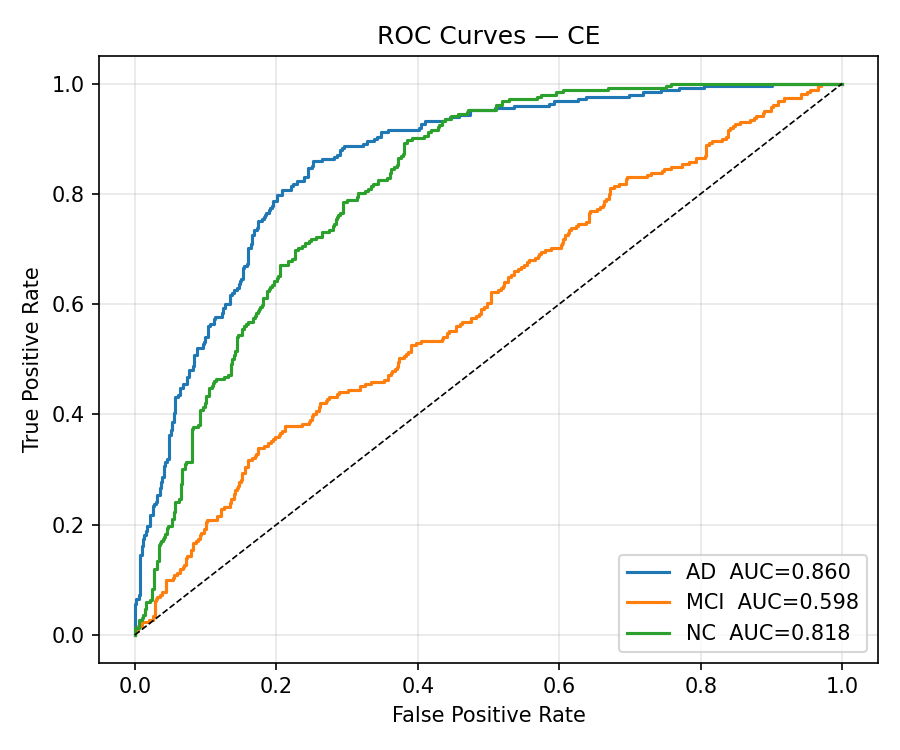
\includegraphics[width=\textwidth]{resnet10/roc_ce.png}
    \caption{ResNet-10 CE}
  \end{subfigure}
  \hfill
  \begin{subfigure}[b]{0.48\textwidth}
    
\includegraphics[width=\textwidth]{resnet18/roc_ce.png}
    \caption{ResNet-18 CE}
  \end{subfigure}
  \caption{ROC curves (one-vs-rest) for the cross-entropy baseline.}
  \label{fig:roc_ce}
\end{figure}

\subsection{Supervised Contrastive}

\begin{figure}[h]
  \centering
  \begin{subfigure}[b]{0.48\textwidth}
    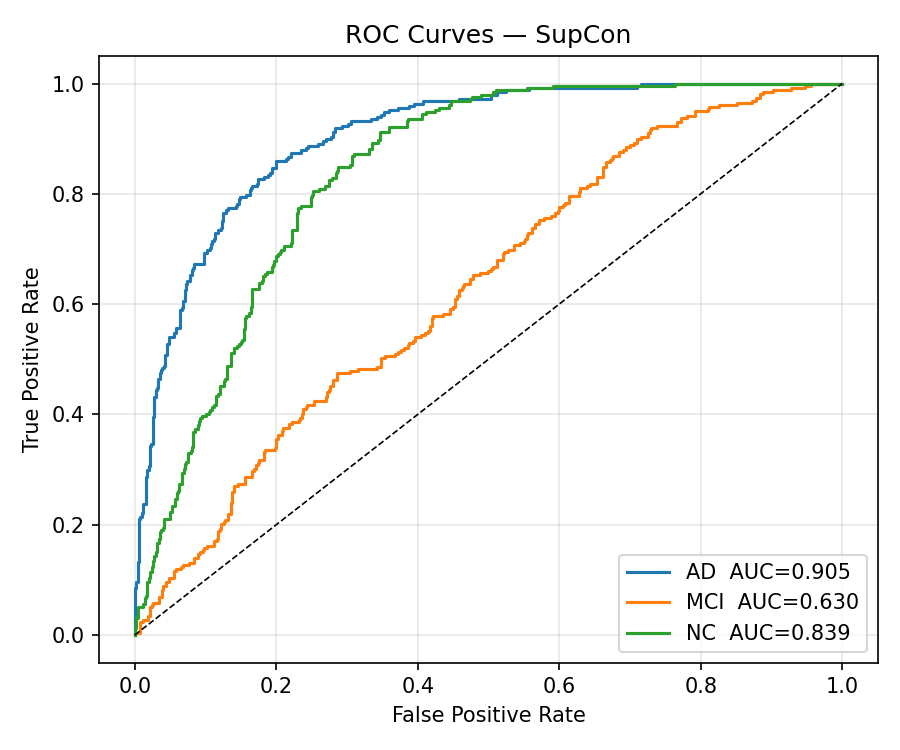
\includegraphics[width=\textwidth]{resnet10/roc_supcon.png}
    \caption{ResNet-10 SupCon}
  \end{subfigure}
  \hfill
  \begin{subfigure}[b]{0.48\textwidth}
    
\includegraphics[width=\textwidth]{resnet18/roc_supcon.png}
    \caption{ResNet-18 SupCon}
  \end{subfigure}
  \caption{ROC curves (one-vs-rest) for supervised contrastive training.}
  \label{fig:roc_supcon}
\end{figure}

\end{document}
